\documentclass[11pt]{exam}
\usepackage{amsfonts}
\usepackage{physics}
\usepackage{cases}
\usepackage{algorithm}
\usepackage{enumitem}
\usepackage{graphicx}
\usepackage{cite}
\usepackage{amsthm,amsmath,amssymb,amsfonts,bm,physics}
\usepackage{array}
\usepackage{upgreek}
\usepackage{algorithmic}
\usepackage{xcolor}
\usepackage{bbm}
\usepackage{booktabs}
\usepackage{multirow}
\usepackage[hidelinks]{hyperref}
\newcommand*\widefbox[1]{\fbox{\hspace{2em}#1\hspace{2em}}}

\newcommand{\gr}{\selectlanguage{greek}}

%\newcommand{\red}{\color{myred}}
%\newcommand{\blue}{\color{myblue}}
%\newcommand{\black}{\color{myblack}}


%\definecolor{BrickRed}{cmyk}{0,0.89,0.94,0.28}
%\definecolor{pink}{RGB}{255,192,203}

\begin{document}
\centerline{\Large \sc Homework 9}
\pagestyle{empty}

\hrulefill

\vspace{2cm}


{\Large \sc Name:}



\vspace{2cm}



{\Large \sc Student ID:}

\vspace{6cm}

\begin{itemize}
  \item Reasoning and work must be shown to gain partial/full
  credit
  \item Please include the cover-page on your homework PDF with your name and student ID. Failure of doing so is considered bad citizenship. 

 \end{itemize}

\clearpage



\begin{questions}
\question[2]{\bf Revise final project}:
Start a preliminary document, using the template \href{https://www.overleaf.com/latex/templates/ieee-conference-template/grfzhhncsfqn}{IEEE Conference on overleaf} for your final project.  
Update the plan, breaking it in tasks and documenting it in the two column paper as follows: 
\begin{description}
\item[Abstract] Write a short description in the abstract. 
\item[Introduction] Expand with a motivation, state what you want to do again as in the abstract and refer to previous work from the literature. 
\item[Problem formulation] Write down a mathematical model and/or description of your problem.
\item[Proposed Approach] In here, you will want to propose what you want to do, broken down in tasks
\item[Analysis and numerical results] The fourth section should be having charts, tables etc. that document numerical results. While you will finish at the end of the course, You should visualize one simple numerical results that shows you are set to succeed in your final project, and that should be illustrative of the preliminary tasks of the proposed approach (e.g. you acquired the data and they make sense).  
\end{description}
\newpage
\question[8]{\bf Network embeddings}: In this problem, you will use two types of network embeddings to cluster the nodes of a transportation network. In particular, we will use the driving network of Manhattan, provided in the files \textit{nodes.csv} and \textit{streets.csv}, and shown below. (\textit{The python package OSMnx\footnote{https://osmnx.readthedocs.io/en/stable/}  lets you download geospatial data from OpenStreetMap and model, project, visualize, and analyze real-world street networks and any other geospatial geometries})
\begin{figure}[ht]
  \centering
  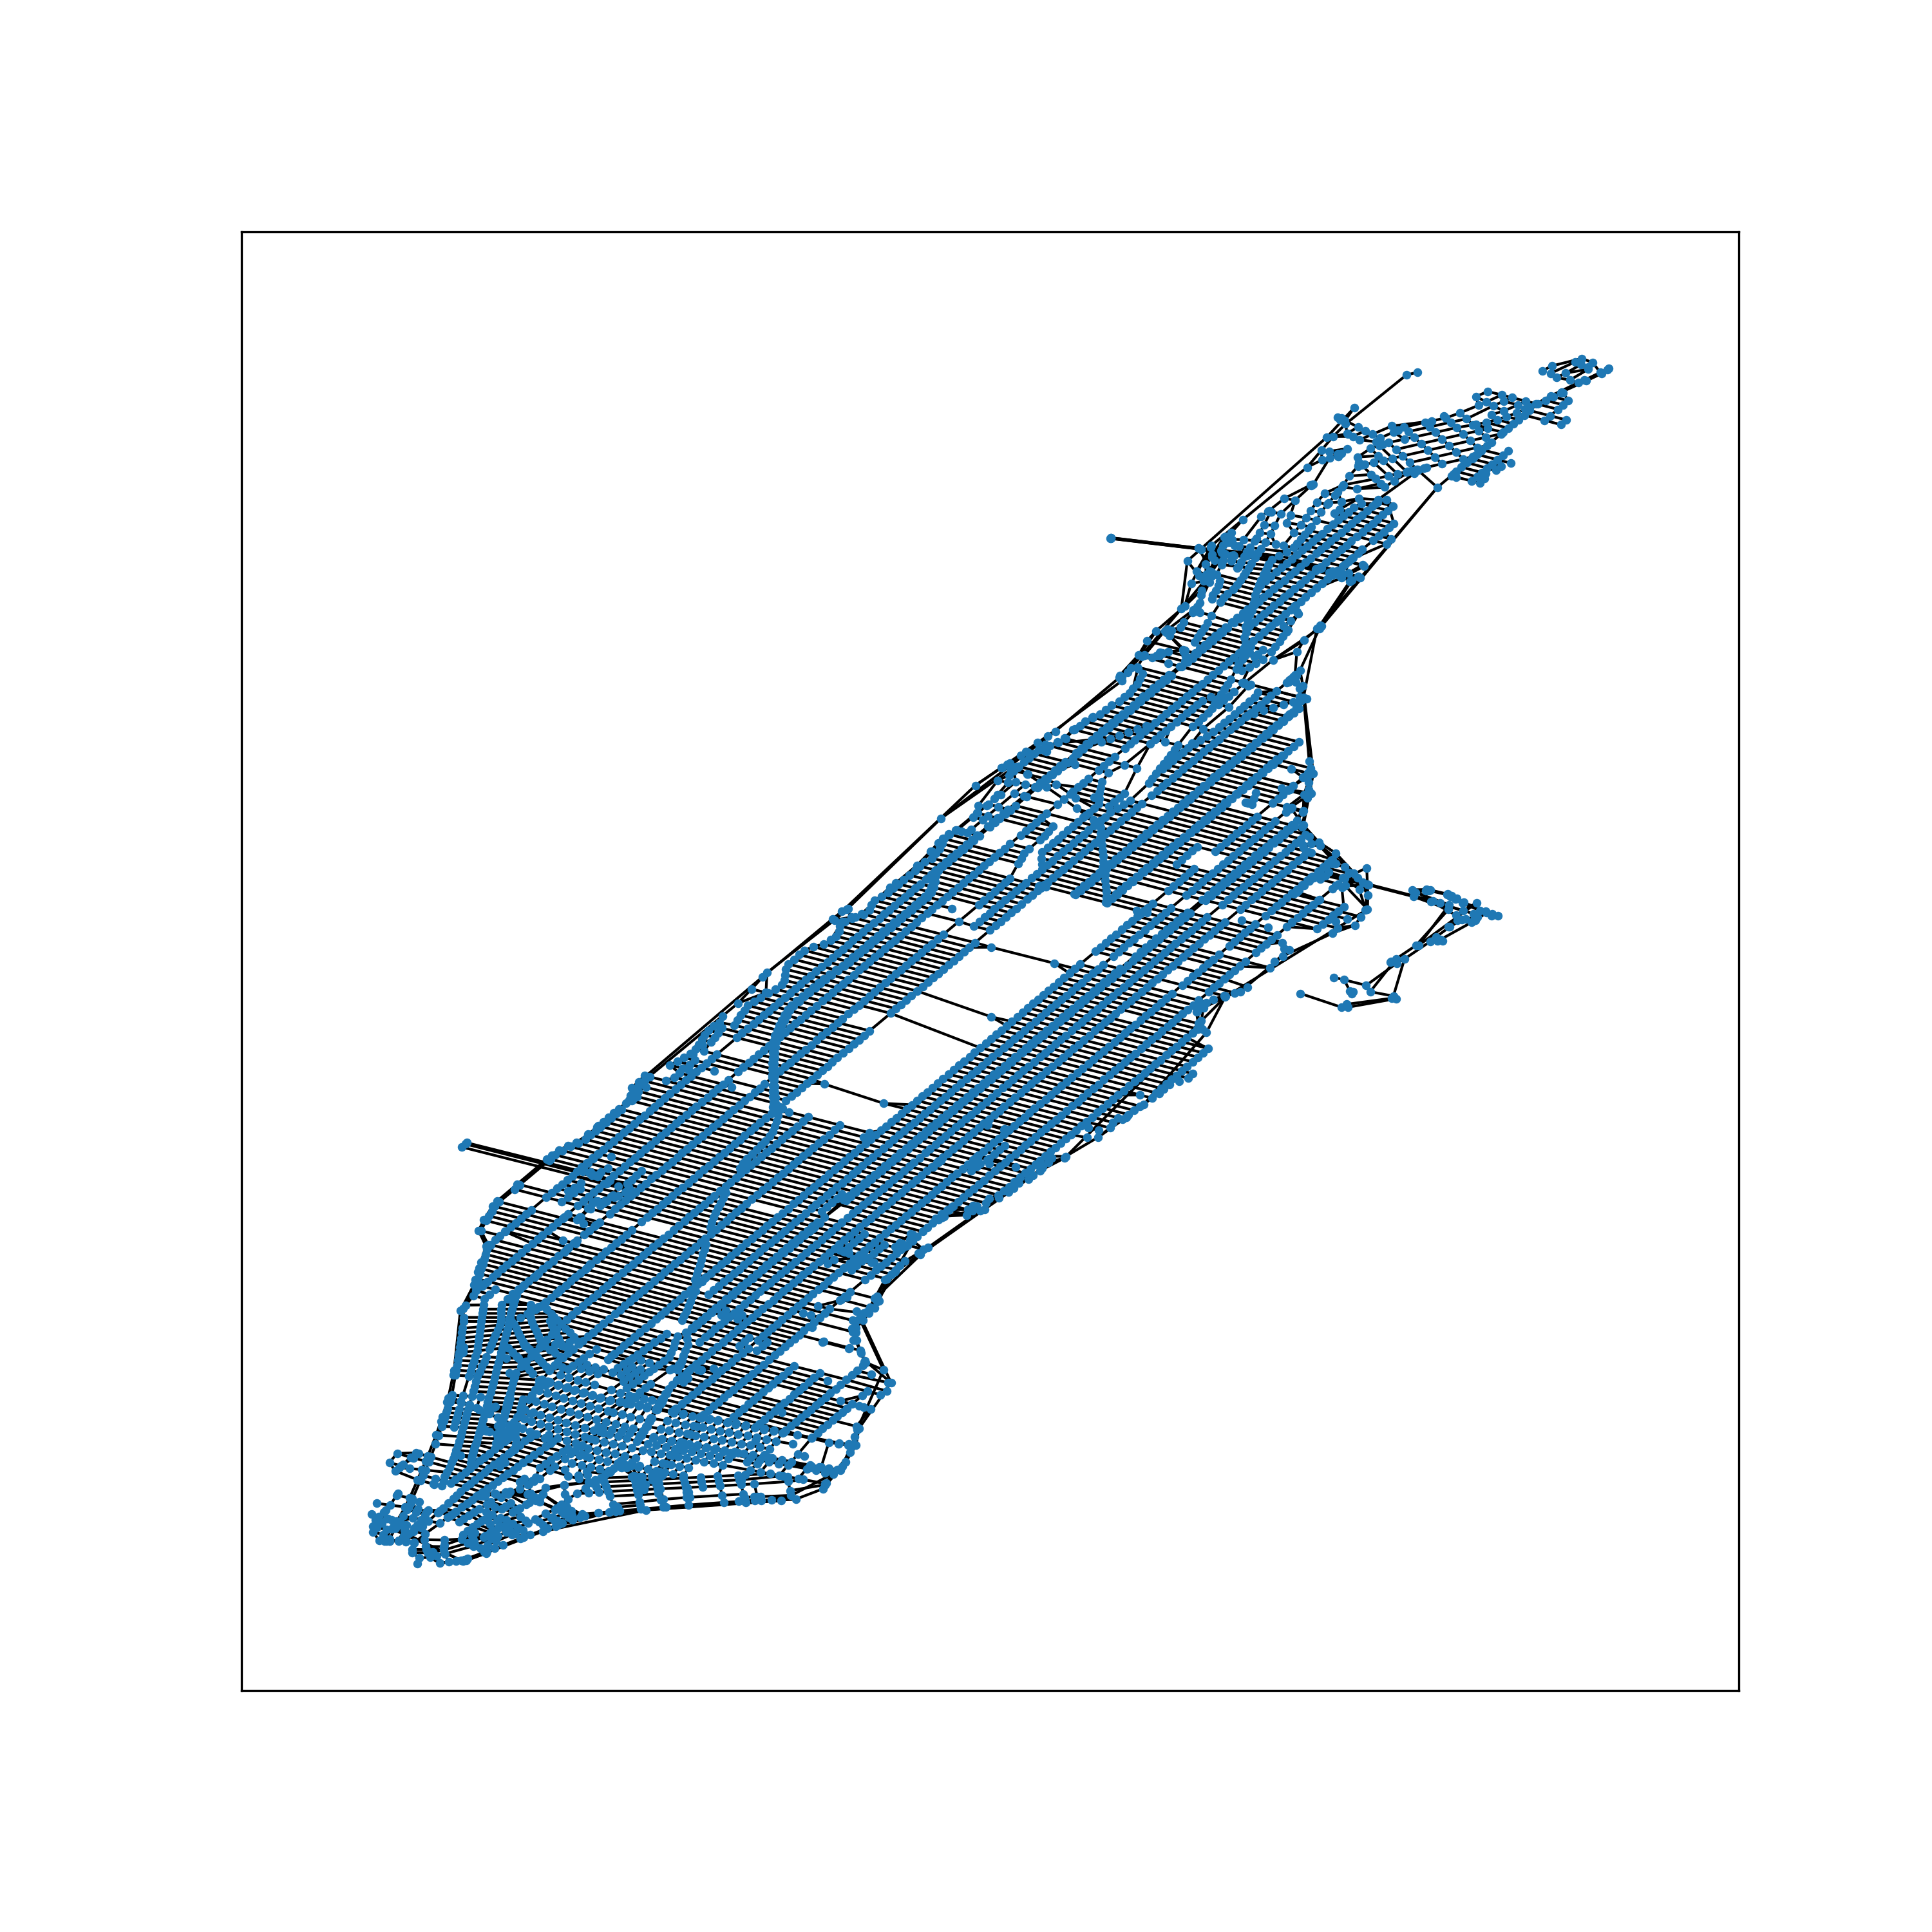
\includegraphics[width = 0.5\textwidth]{../manhattan.png}
  \vspace{-1cm}
  \caption{Manhattan driving network}
  \label{fig:manhattan}
\end{figure}
\begin{parts}
  \part[1] Build the driving network in networkx and use the distance between nodes as the weight of each edge.
  \part[1] Remove the self loops using the function \textit{G.remove\_edges\_from(nx.selfloop\_edges(G))} and plot the network using the coordinates of each node as its position (similar to Fig. \ref{fig:manhattan} but with a different color for the nodes).
  \part[3] \textbf{skip2gram approach} Apply the Node2Vec algorithm to the graph (You may rely on the python implementation Node2Vec\footnote{https://github.com/eliorc/node2vec}) (\textbf{Hint}: You may want to use the following hyperparameters \textit{dimensions=32}, \textit{walk\_length=50}, \textit{num\_walks=300},\textit{window=10}, \textit{min\_count=1}, \textit{batch\_words=4}. Also, Node2Vec will not return the embeddings in order. Please take this into consideration for the following sections.)
  \part[1] \textbf{Matrix factorization} Obtain the eigendecomposition of the weighted Laplacian.
  \part[1] Plot the network embeddings from (c) and (d) in 2D using some dimensionality reduction method (e.g. PCA, TSNE). What do you observe?
  \part[1] Using the results from (c) and (d), cluster the network using using Kmeans. For the number of clusters, use 32 clusters. To validate your results, load the shapefile \textit{manhattan.shp} that contains the neighborhoods of Manhattan, and overlay your results (use geopandas\footnote{https://geopandas.org/en/stable/} to plot the shapefile). Use a different color for each cluster, and comment your results.
\end{parts}
    


\end{questions}





\end{document}




